\documentclass[aspectratio=43]{beamer}
\usetheme{Berlin}

\title{Sample Title}
\subtitle{Sample Subtitle}
\usepackage[czech]{babel}
\usecolortheme{dolphin}
\usepackage{graphicx}
\usepackage{dirtree}
\usepackage{listings}
\usepackage[utf8]{inputenc}
\usepackage{caption}		% popisky

\captionsetup{labelformat=empty}

\defbeamertemplate*{title page}{customized}[1][]
{
	\usebeamerfont{title}\inserttitle\par
	\usebeamerfont{subtitle}\usebeamercolor[fg]{subtitle}\insertsubtitle\par
	\bigskip
	\usebeamerfont{author}\insertauthor\par
	\usebeamerfont{institute}\insertinstitute\par
	\usebeamerfont{date}\insertdate\par
	\usebeamercolor[fg]{titlegraphic}\inserttitlegraphic
}

\hypersetup{unicode}
\hypersetup{breaklinks=true}

\usepackage{color}
\definecolor{pblue}{rgb}{0.13,0.13,1}
\definecolor{pgreen}{rgb}{0,0.5,0}
\definecolor{pred}{rgb}{0.9,0,0}
\definecolor{pgrey}{rgb}{0.46,0.45,0.48}




\title{Linux Manager}
\subtitle{Závěrečná práce}
\author{Havránek Kryštof 3.E}
\date{16. června 2021}
\institute{Gymnázium, Arabská 14, Praha 6}
\setbeamertemplate{sidebar right}{}
\setbeamertemplate{footline}{%
\hfill\textbf{\insertframenumber{}/\inserttotalframenumber}}


\begin{document}
\begin{frame}[plain]
	\maketitle
\end{frame}
\frame{
	\frametitle{Úvod}
	\section{Úvod}
	\begin{itemize}
		\item Sledování stavu několika počítačů
		\item Node.js
		\item React.js, Redux, Bluma, Ramda
		\item Boilerplate
	\end{itemize}

}
\frame{
	\frametitle{Funkce}
	\section{Funkce}
	\begin{itemize}
		\item Sledování základních údajů
		\item Package, které lze updatovat
		\item Graf historie zátěže CPU a RAM
	\end{itemize}
}

\frame{
	\frametitle{Architektura}
	\section{Architektura}
	\centering
	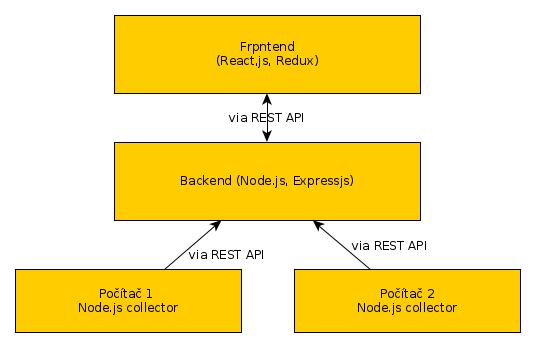
\includegraphics[height=6cm]{./5 - Program Structure.jpg} % websocket
}
\end{document}
